\section{Introduction}
\label{sec:introduction}

Quantum cognition models judgment, memory, and decision making with the
mathematical structure of quantum probability. It does not claim that the brain
is a quantum computer. Instead, it uses Hilbert spaces, superposition, and
interference to capture contextuality, order effects, and evidence accumulation
that classical probability handles awkwardly \citep{pothos2022,busemeyer2024}.
Quantum walks are a natural process-level ingredient: a walker on a semantic or
decision graph represents unfolding evidence, a marked vertex represents a
target memory or an option, and the walk's statistics define response times and
choice probabilities \citep{chen2022,huang2022,pavone2025}.

The missing link is algorithmic structure. The quantum-walk literature on
search focuses on worst-case query and time complexity: given a graph and a
marked set, how quickly can one detect or find a marked vertex? The quantum
cognition literature focuses on explaining behavioral signatures. The two
bodies of work meet mostly through the metaphor that a quantum walk is an
evidence accumulator. The marked-vertex search problem itself---especially its
behavior with multiple marked vertices---is rarely used as a formal model of
cognitive search.

This project uses the Ambainis--Gily\'en--Jeffery--Kokainis (AGJK) algorithm as
the technical core \citep{agjk2019}. AGJK gives a quantum walk algorithm that
finds a marked vertex on an arbitrary graph, for an arbitrary marked set, with
a quadratic speedup over the classical hitting time up to logarithmic factors.
It also isolates the extended hitting time $\HT^+$, which can be much larger
than $\HT$ when there are multiple marked vertices. That structure maps
naturally onto cognitive search with several targets and onto multi-alternative
choice, where similar options compete and context changes the choice
distribution.

We ask three questions.
\begin{enumerate}[leftmargin=1.4em]
  \item \textbf{Mapping.} How do $\HT$, $\HT^+$, the spectral gap, and the
  success probability map onto response time, choice probability, and
  deliberation speed on a semantic or decision graph?
  \item \textbf{Structure.} How do the number and arrangement of marked
  vertices---single, independent, clustered---change the quantum versus
  classical search time and success probability? Can $\HT^+$ formalize
  multi-alternative decision difficulty and context effects?
  \item \textbf{Noise.} How does partial measurement or decoherence erode the
  quantum advantage, and is there an optimal ``introspection'' level that
  maximizes success probability or decision speed?
\end{enumerate}

\Cref{fig:architecture} summarizes the three layers of the project: the QIS
core, the graph model, and the cognitive quantities derived from the walk.

\begin{figure}[t]
  \centering
  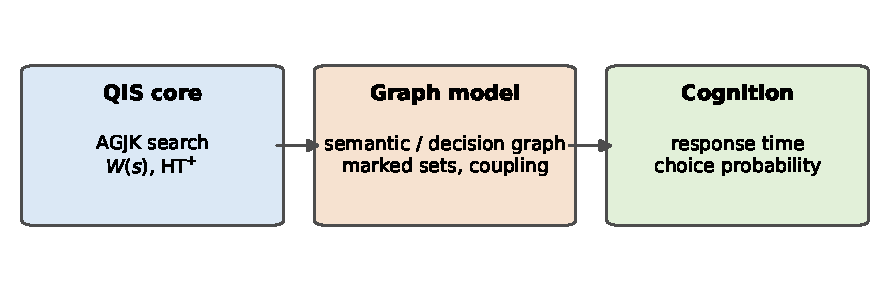
\includegraphics[width=0.92\linewidth]{figures/fig_architecture.pdf}
  \caption{Three-layer architecture. The AGJK search core supplies the walk
  operator and the hitting-time structure; the graph layer maps concepts or
  options to vertices and marked sets; the cognitive layer turns walk statistics
  into response times and choice probabilities.}
  \label{fig:architecture}
\end{figure}

The project makes four contributions. First, we implement the Szegedy walk,
the interpolated walk $W(s)$, and the AGJK extended hitting time, and we verify
the $\widetilde O(\sqrt{\HT})$ scaling numerically on complete graphs, cycles,
grids, and hypercubes. Second, we compare single, independent, and clustered
marked sets. We show that independent targets are easier, that clustered
targets give only a modest reduction of the hitting time relative to a single
target ($\approx3\%$ on the barbell, $\approx17\%$ on the $8\times8$ grid), and that the dramatic $\HT^+\gg\HT$ gap
requires the adversarial periodic arrangement of AGJK rather than clustering
alone. Third, we build a semantic graph and a multi-branch decision graph and
turn the walk statistics into target activation, response time, and choice
probability. Fourth, we add a partial-measurement model and show that
single-deadline comparisons are dominated by the phase of the quantum
oscillation. With deadline-free readouts, the pure walk keeps the highest timed
peak, while at moderate deadlines an intermediate measurement rate that can
stop the search finds clustered targets faster than both the pure quantum and
the classical walk.

The paper is organized as follows. \Cref{sec:background} reviews classical and
quantum walks and the quantum cognition literature. \Cref{sec:theory} collects
the formal definitions and the AGJK results we use. \Cref{sec:cognitive-model}
states the cognitive mapping and its assumptions. \Cref{sec:methods} describes
the graph families, protocols, and metrics. \Cref{sec:results} reports E1--E5.
\Cref{sec:discussion} discusses interpretation, limitations, and future work.
